\chapter{THIẾT KẾ VÀ XÂY DỰNG CHƯƠNG TRÌNH MATLAB}
\section{Tổng quan cấu trúc chương trình}
% TODO: dán nội dung từ Google Docs vào đây.

\section{Ứng dụng Symbolic Math Toolbox}
% TODO: dán nội dung từ Google Docs vào đây.

\section{Thuật toán tính toán số trị}
% TODO: dán nội dung từ Google Docs vào đây.

\section{Thiết kế giao diện và vẽ quỹ đạo}
% TODO: dán nội dung từ Google Docs vào đây.

% Ví dụ chèn hình (file nằm trong ../figures/):
% \begin{figure}[H]
%   \centering
%   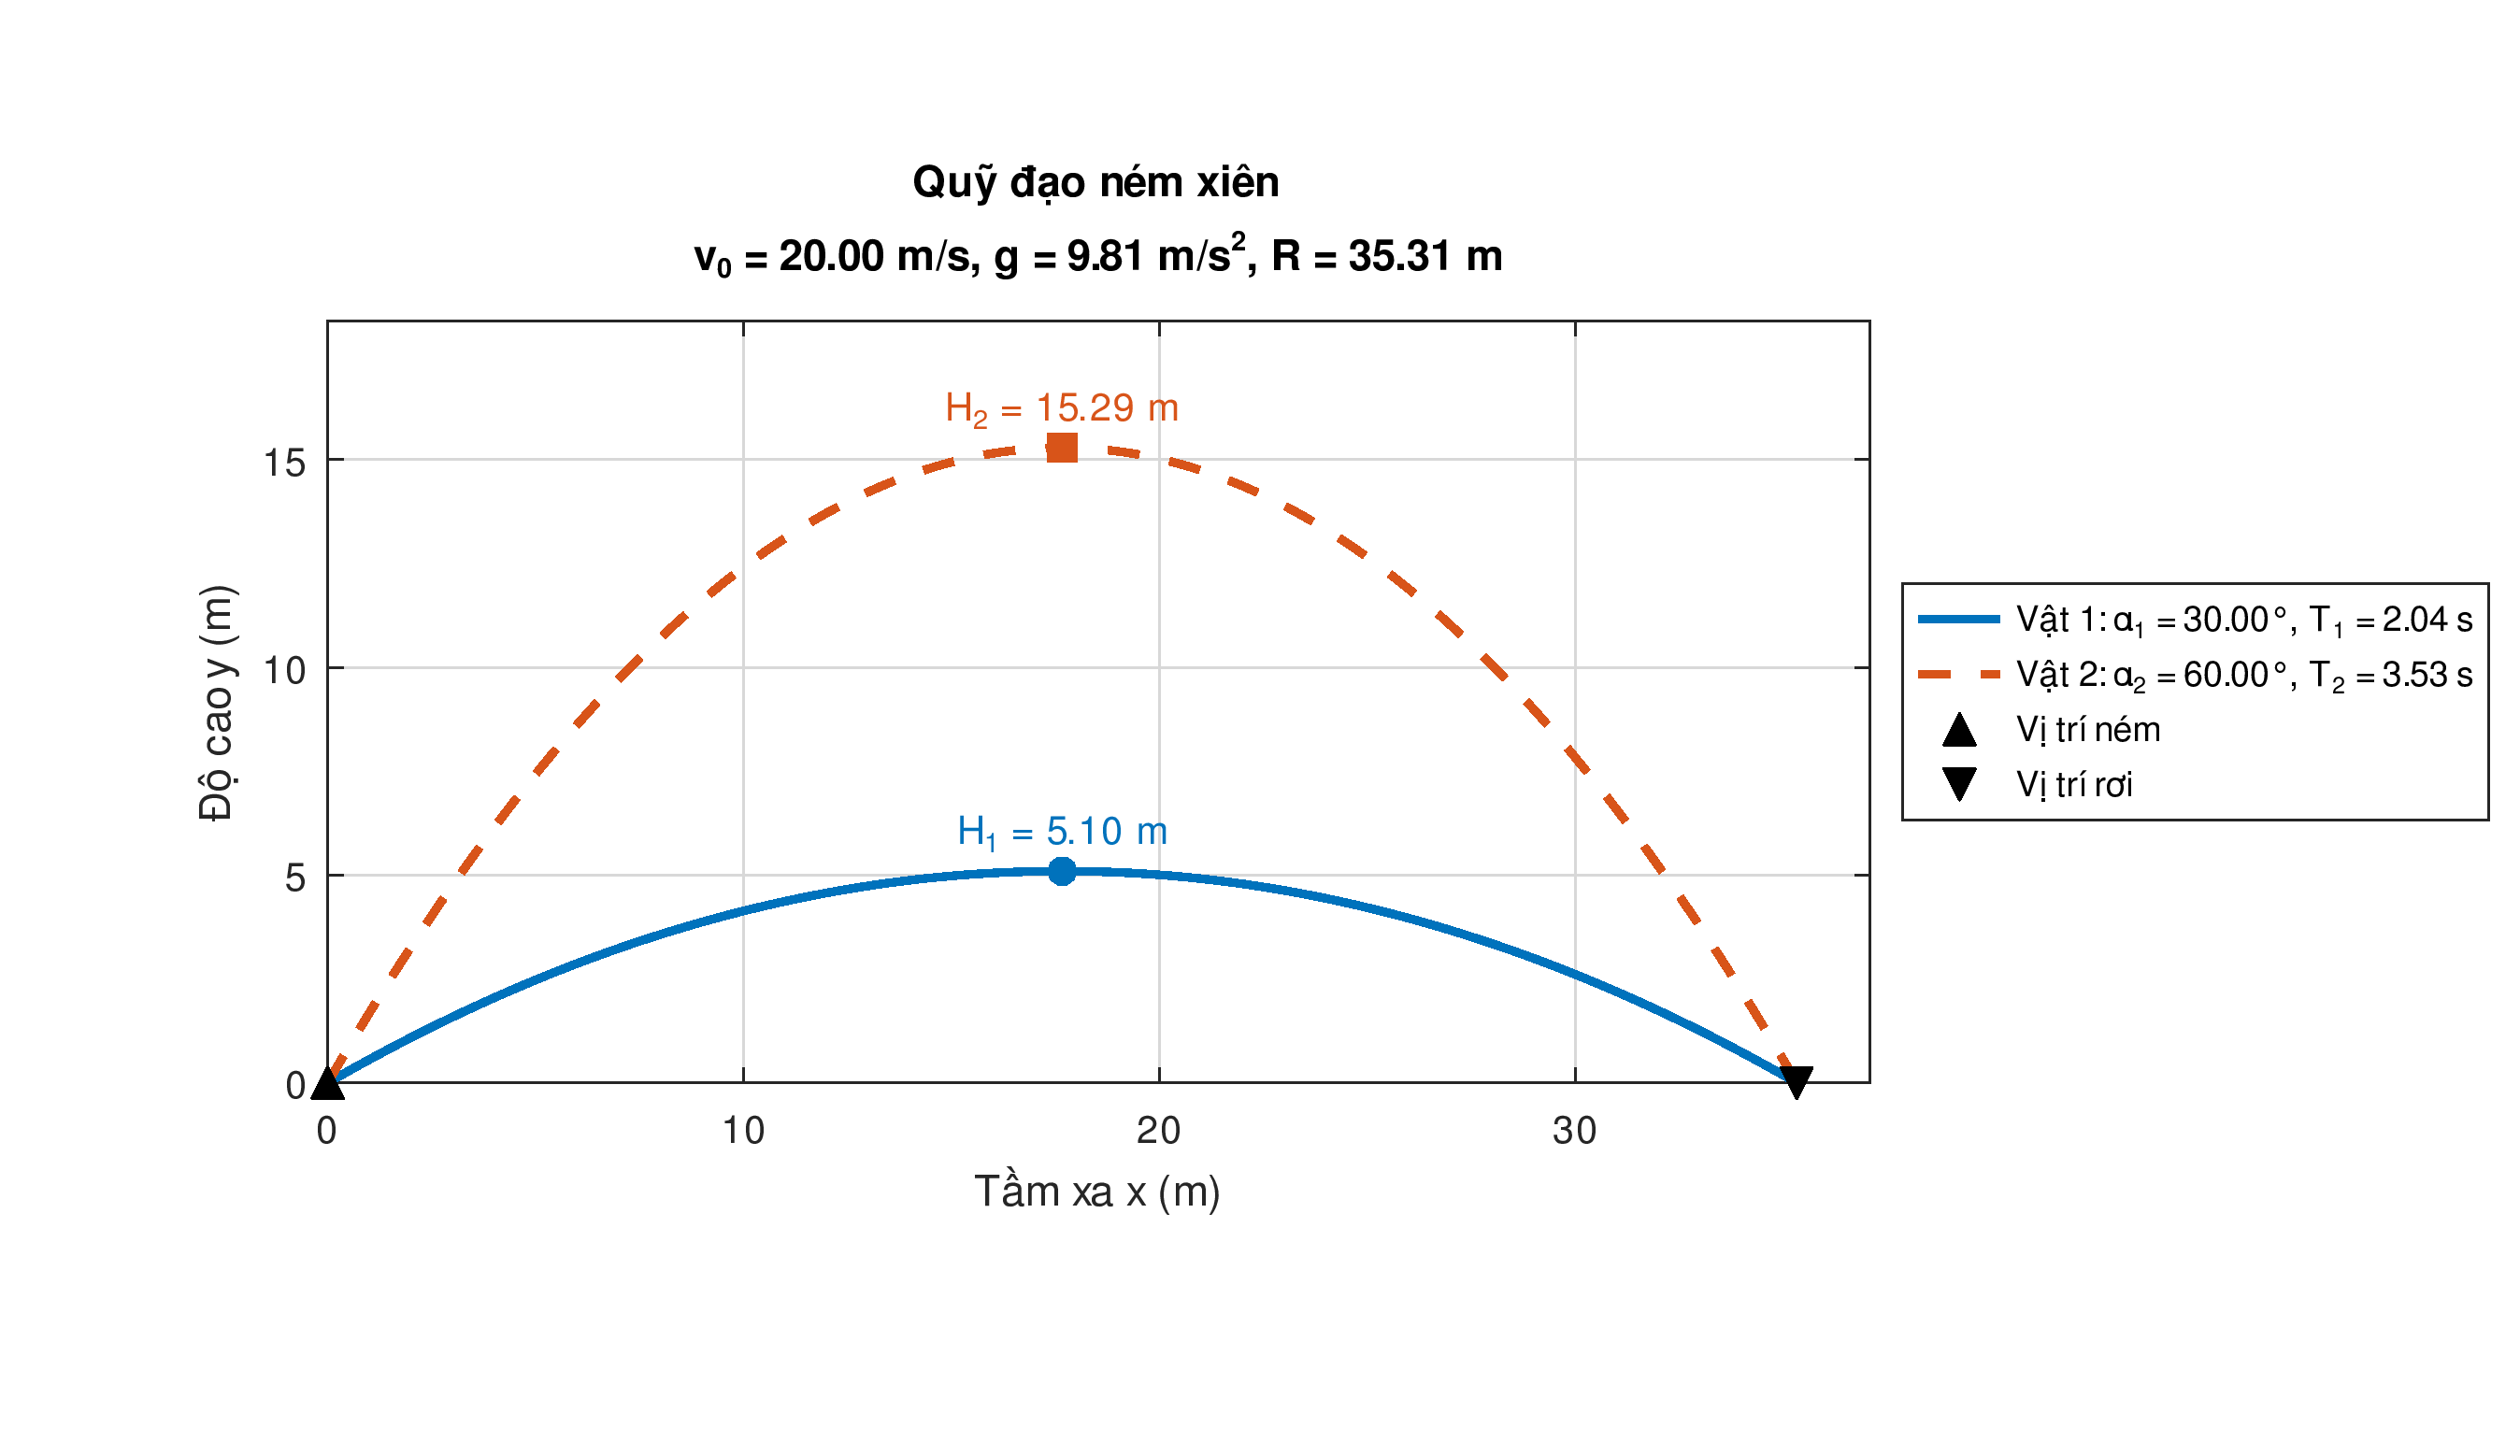
\includegraphics[width=0.9\textwidth]{quydao_v0_20_alpha1_30.png}
%   \caption{Quỹ đạo hai vật với $v_0 = 20$~m/s, $\alpha_1 = 30^\circ$}
%   \label{fig:quydao30}
% \end{figure}
